\documentclass{beamer}

\usetheme{Warsaw}

\usepackage[english]{babel}
\usepackage[utf8]{inputenc}
\usepackage{times}
\usepackage[T1]{fontenc}
\usepackage{xcolor}

\title{The Development of Purdue's Computerized Interactive Teaching Assistant}
\subtitle{Cyrus Vandrevala, Lynn Bryan, Andrew Hirsch, Hisao Nakanishi, Laura Pyrak-Nolte}
\date{August 6, 2015}

\begin{document}

\begin{frame}
  \titlepage
\end{frame}

\begin{frame}
  \tableofcontents
\end{frame}

\section{Background}

\subsection{Introduction}

\begin{frame}{What is CITA?}
  \begin{itemize}
    \item<1-> First bullet point
    \item<2-> Second bullet point
    \item<3-> Third bullet point
  \end{itemize}
\end{frame}

\begin{frame}{Enrollment in Electricity and Optics}
  \begin{figure}
    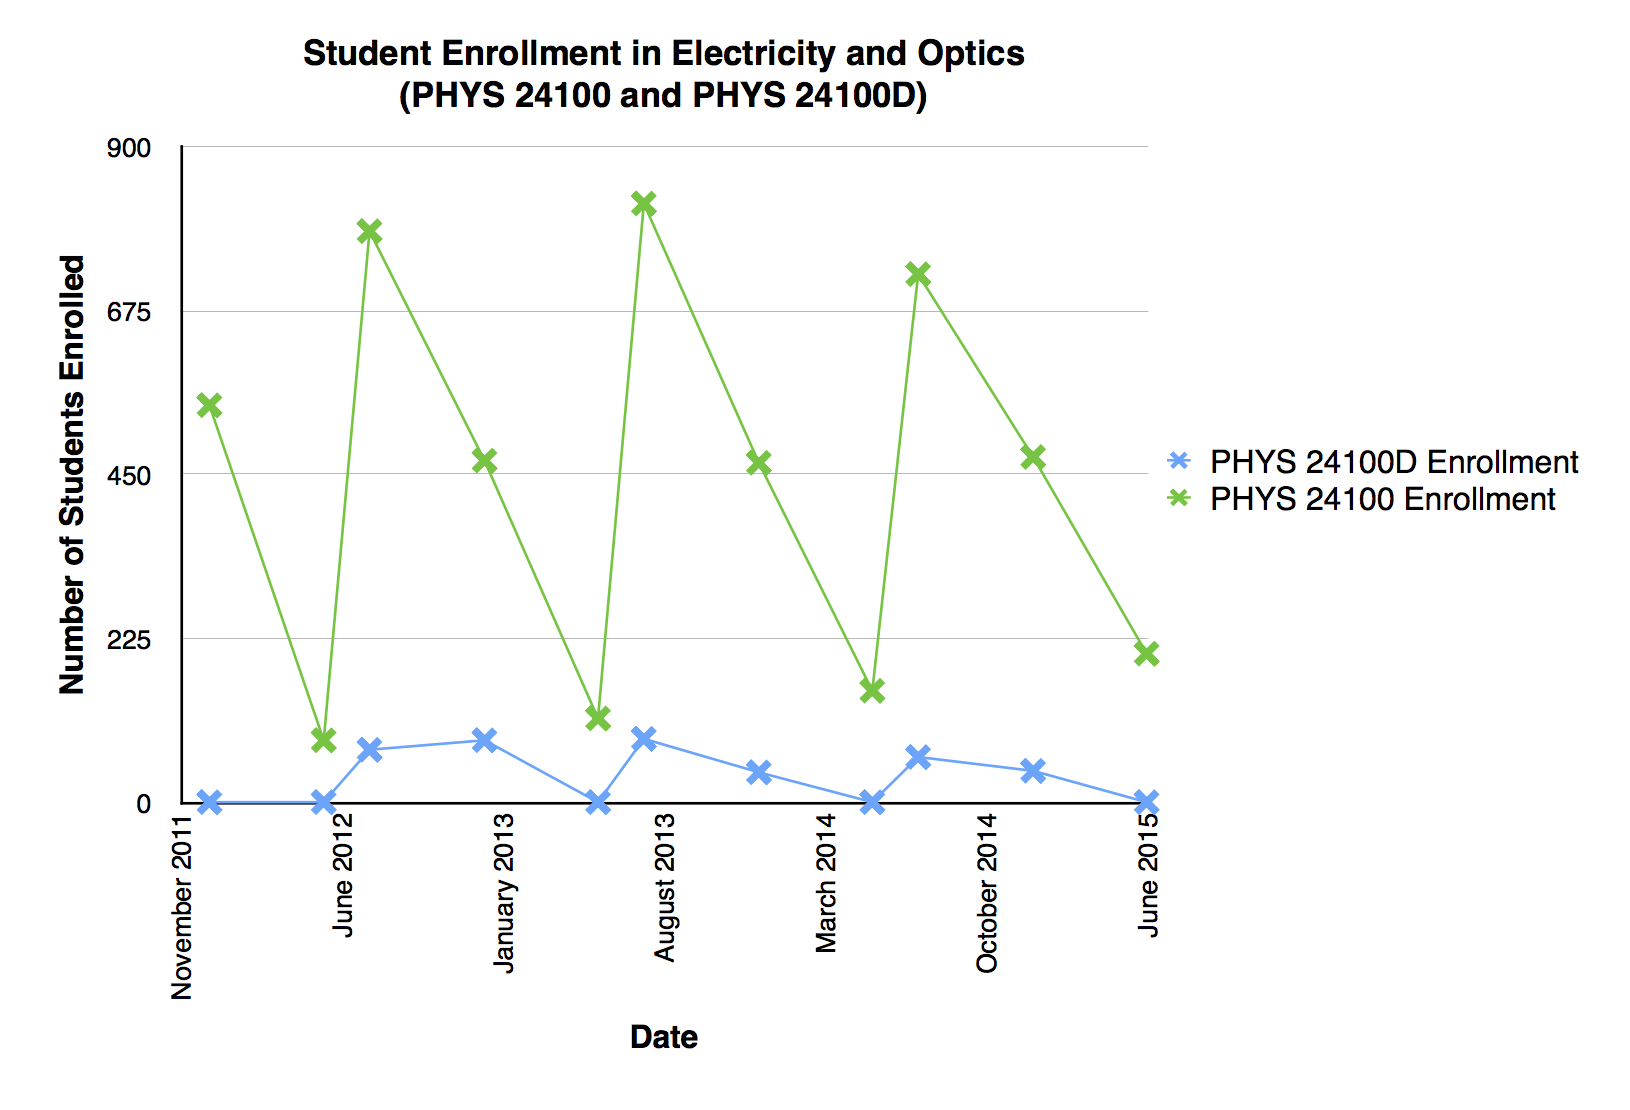
\includegraphics[width=4in]{img/chapter1/enrollment}
  \end{figure}
\end{frame}

\begin{frame}{Enrollment in Electricity and Optics}
  \begin{figure}
    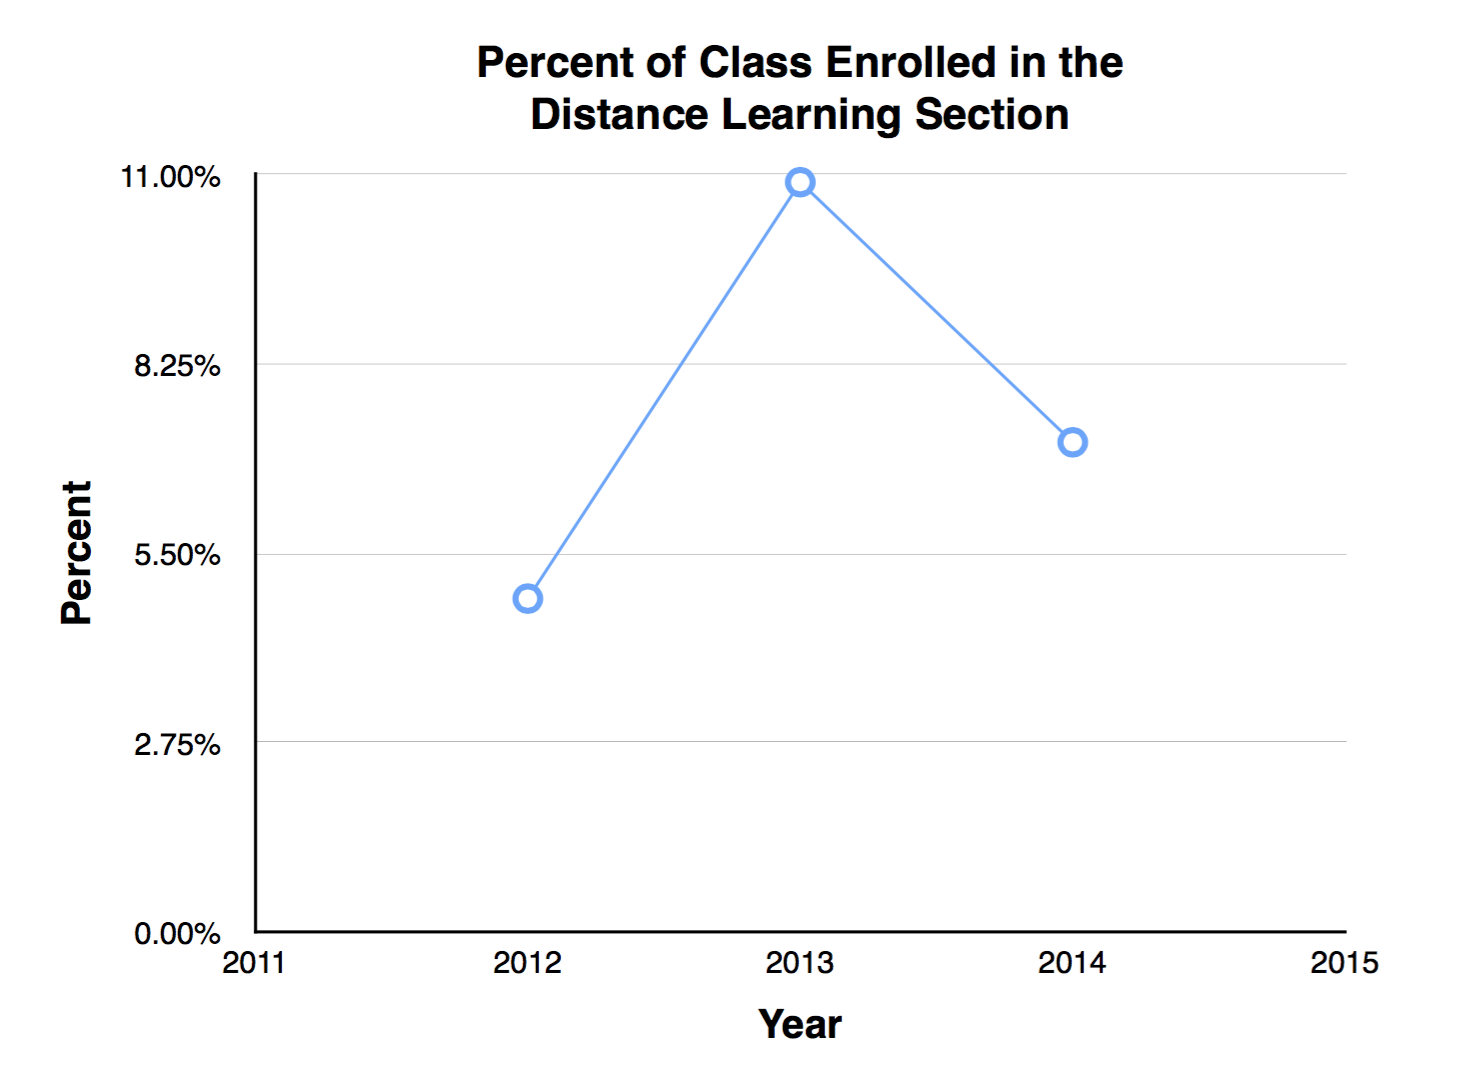
\includegraphics[width=3.5in]{img/chapter1/percent}
  \end{figure}
\end{frame}

\section{The CITA System}

\begin{frame}{What is CITA?}
  We want students to...
  \begin{itemize}
    \item explore problems in different ways.
    \item see the connections between different paths of logic.
    \item discuss their strategies with each other.
    \item learn from their mistakes.
  \end{itemize}
\end{frame}

\begin{frame}{Enrollment in Electricity and Optics}
\begin{columns}
\begin{column}{2in}
\begin{figure}
	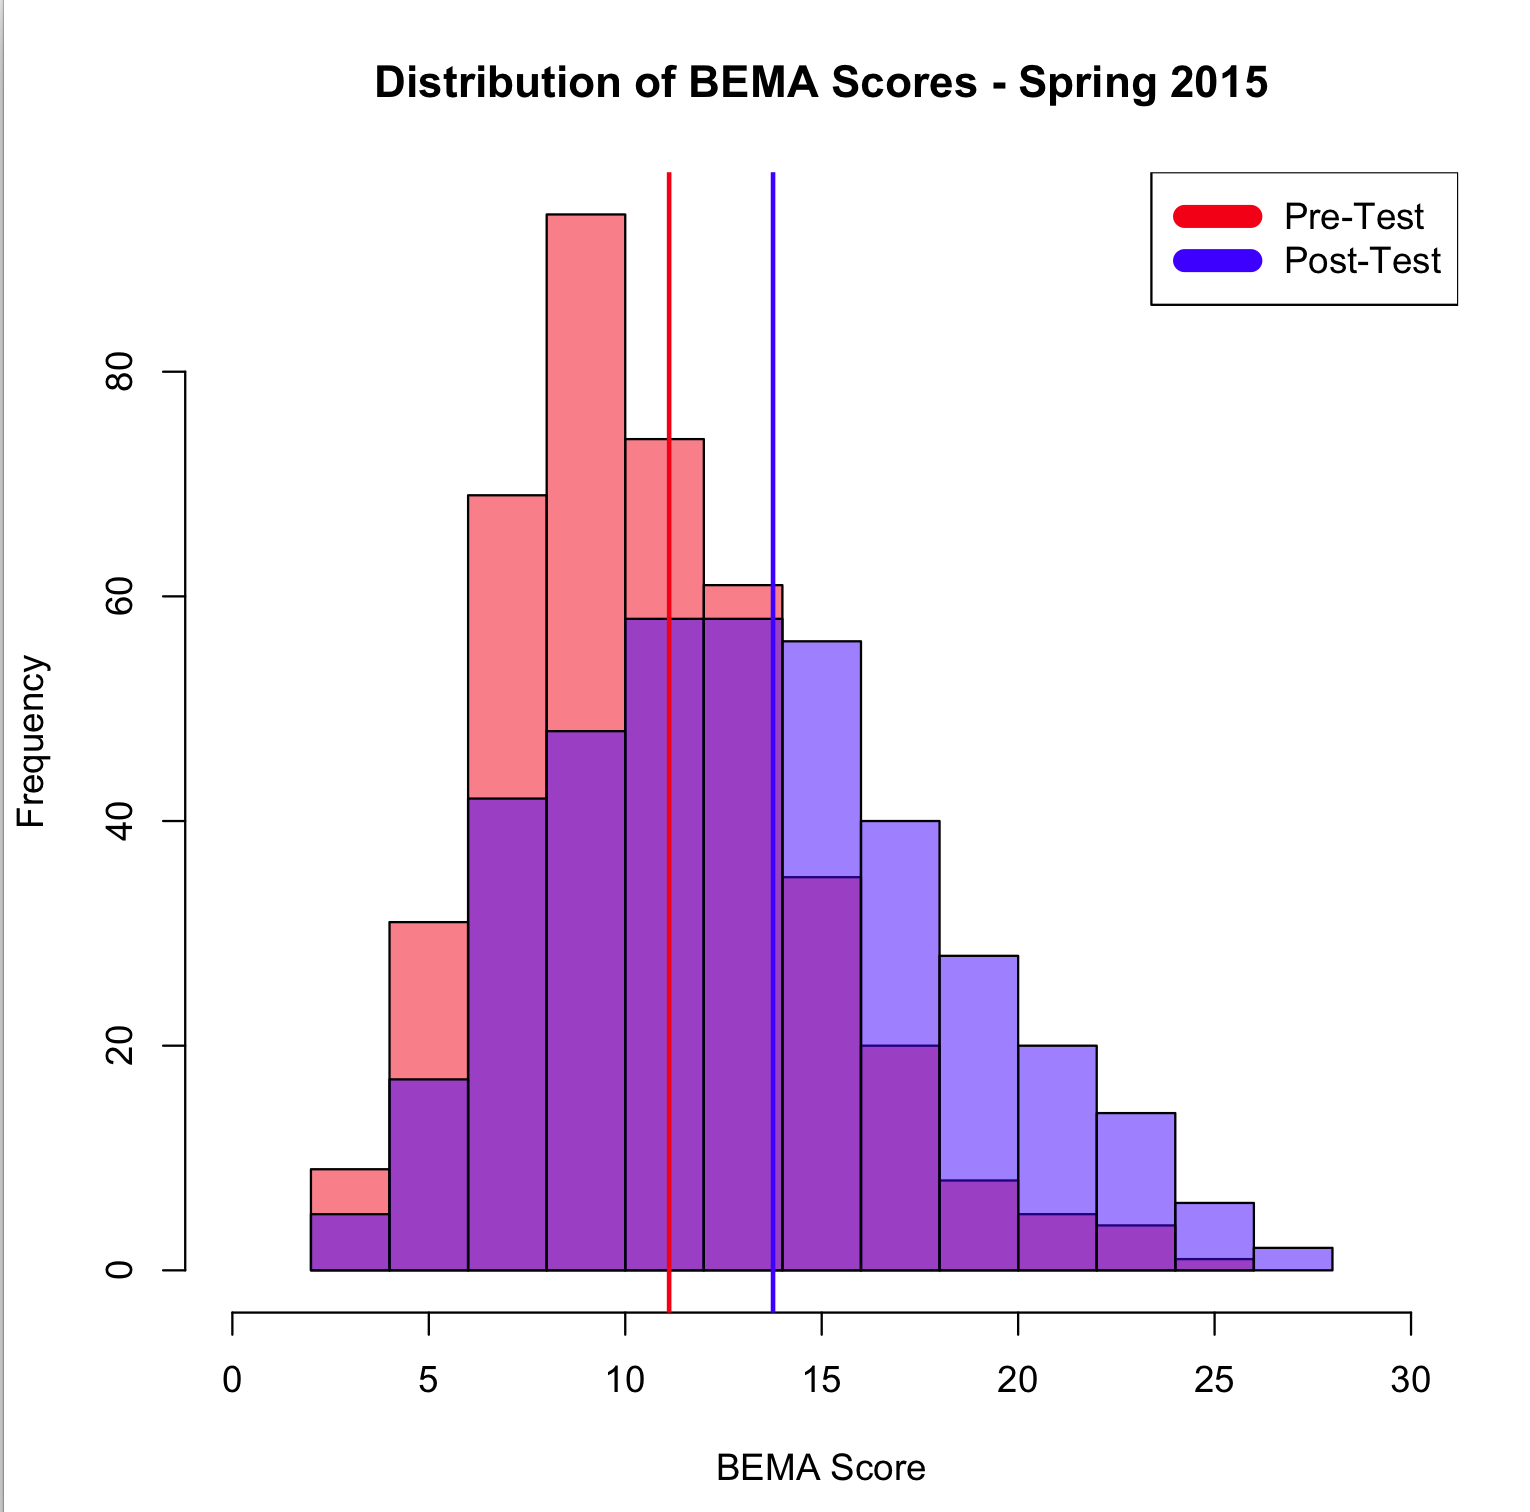
\includegraphics[width=2in]{img/chapter4/bema_spring_2015}
\end{figure}
\end{column}
\begin{column}{2in}
\begin{scriptsize}
\begin{table}
  \centering
  \begin{tabular}{|l|l|}
    \hline
    \textbf{Statistic} & \textbf{Value}\\
	\hline
	$\mu$ - Pre-Test & 11.117 \\
	\hline
	$\mu$ - Post-Test & 13.761 \\
	\hline
	$\sigma$ - Pre-Test & 3.923 \\
	\hline
	$\sigma$ - Post-Test & 5.030 \\
	\hline
	Shapiro-Wilk - Pre-Test & p = 9.24e-08 \\
	\hline
	Shapiro-Wilk - Post-Test & p = 0.000138 \\
	\hline
	Wilcoxon Signed-Rank & p = 9.74e-15 \\
	\hline
	Cohen's D & 0.588 \\
	\hline
  \end{tabular}
\end{table}
\end{scriptsize}
\end{column}
\end{columns}
\end{frame}

\begin{frame}{Enrollment in Electricity and Optics}
\begin{columns}
\begin{column}{2in}
\begin{figure}
	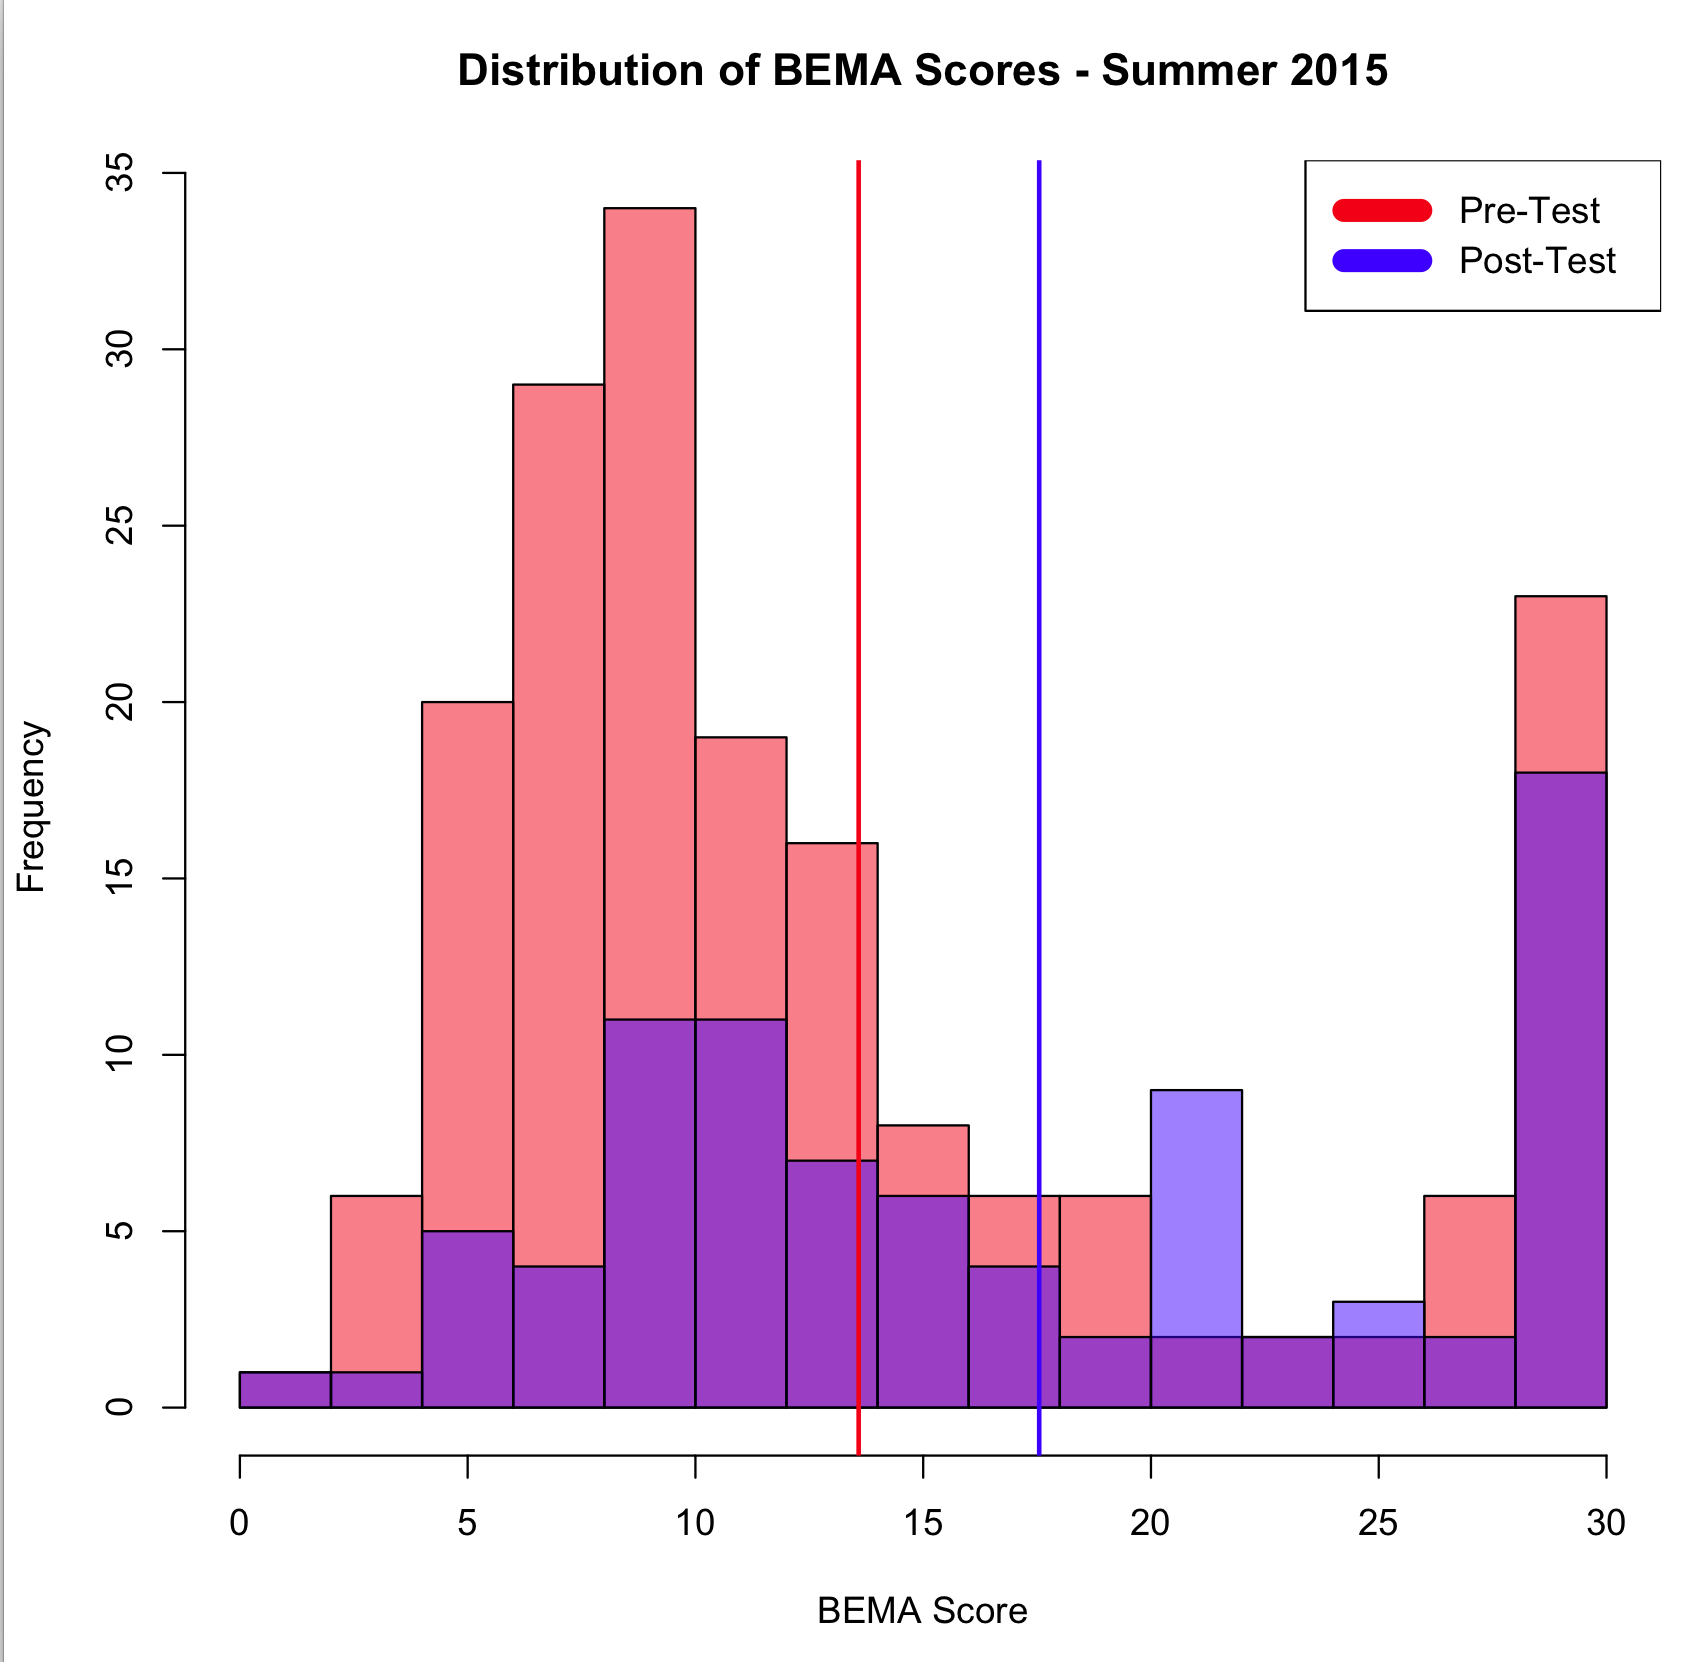
\includegraphics[width=2in]{img/chapter4/bema_summer_2015}
\end{figure}
\end{column}
\begin{column}{2in}
\begin{scriptsize}
\begin{table}
  \centering
  \begin{tabular}{|l|l|}
    \hline
    \textbf{Statistic} & \textbf{Value} \\
	\hline
	$\mu$ - Pre-Test & 13.583 \\
	\hline
	$\mu$ - Post-Test & 17.547 \\
	\hline
	$\sigma$ - Pre-Test & 8.169 \\
	\hline
	$\sigma$ - Post-Test & 8.500 \\
	\hline
	Shapiro-Wilk - Pre-Test & p = 1.599e-12 \\
	\hline
	Shapiro-Wilk - Post-Test & p = 1.332e-05 \\
	\hline
	Wilcoxon Signed-Rank & p = 4.916e-05 \\
	\hline
	Cohen's D & 0.479 \\
	\hline
  \end{tabular}
\end{table}
\end{scriptsize}
\end{column}
\end{columns}
\end{frame}

\begin{frame}{Enrollment in Electricity and Optics}
\begin{columns}
\begin{column}{2in}
\begin{figure}
	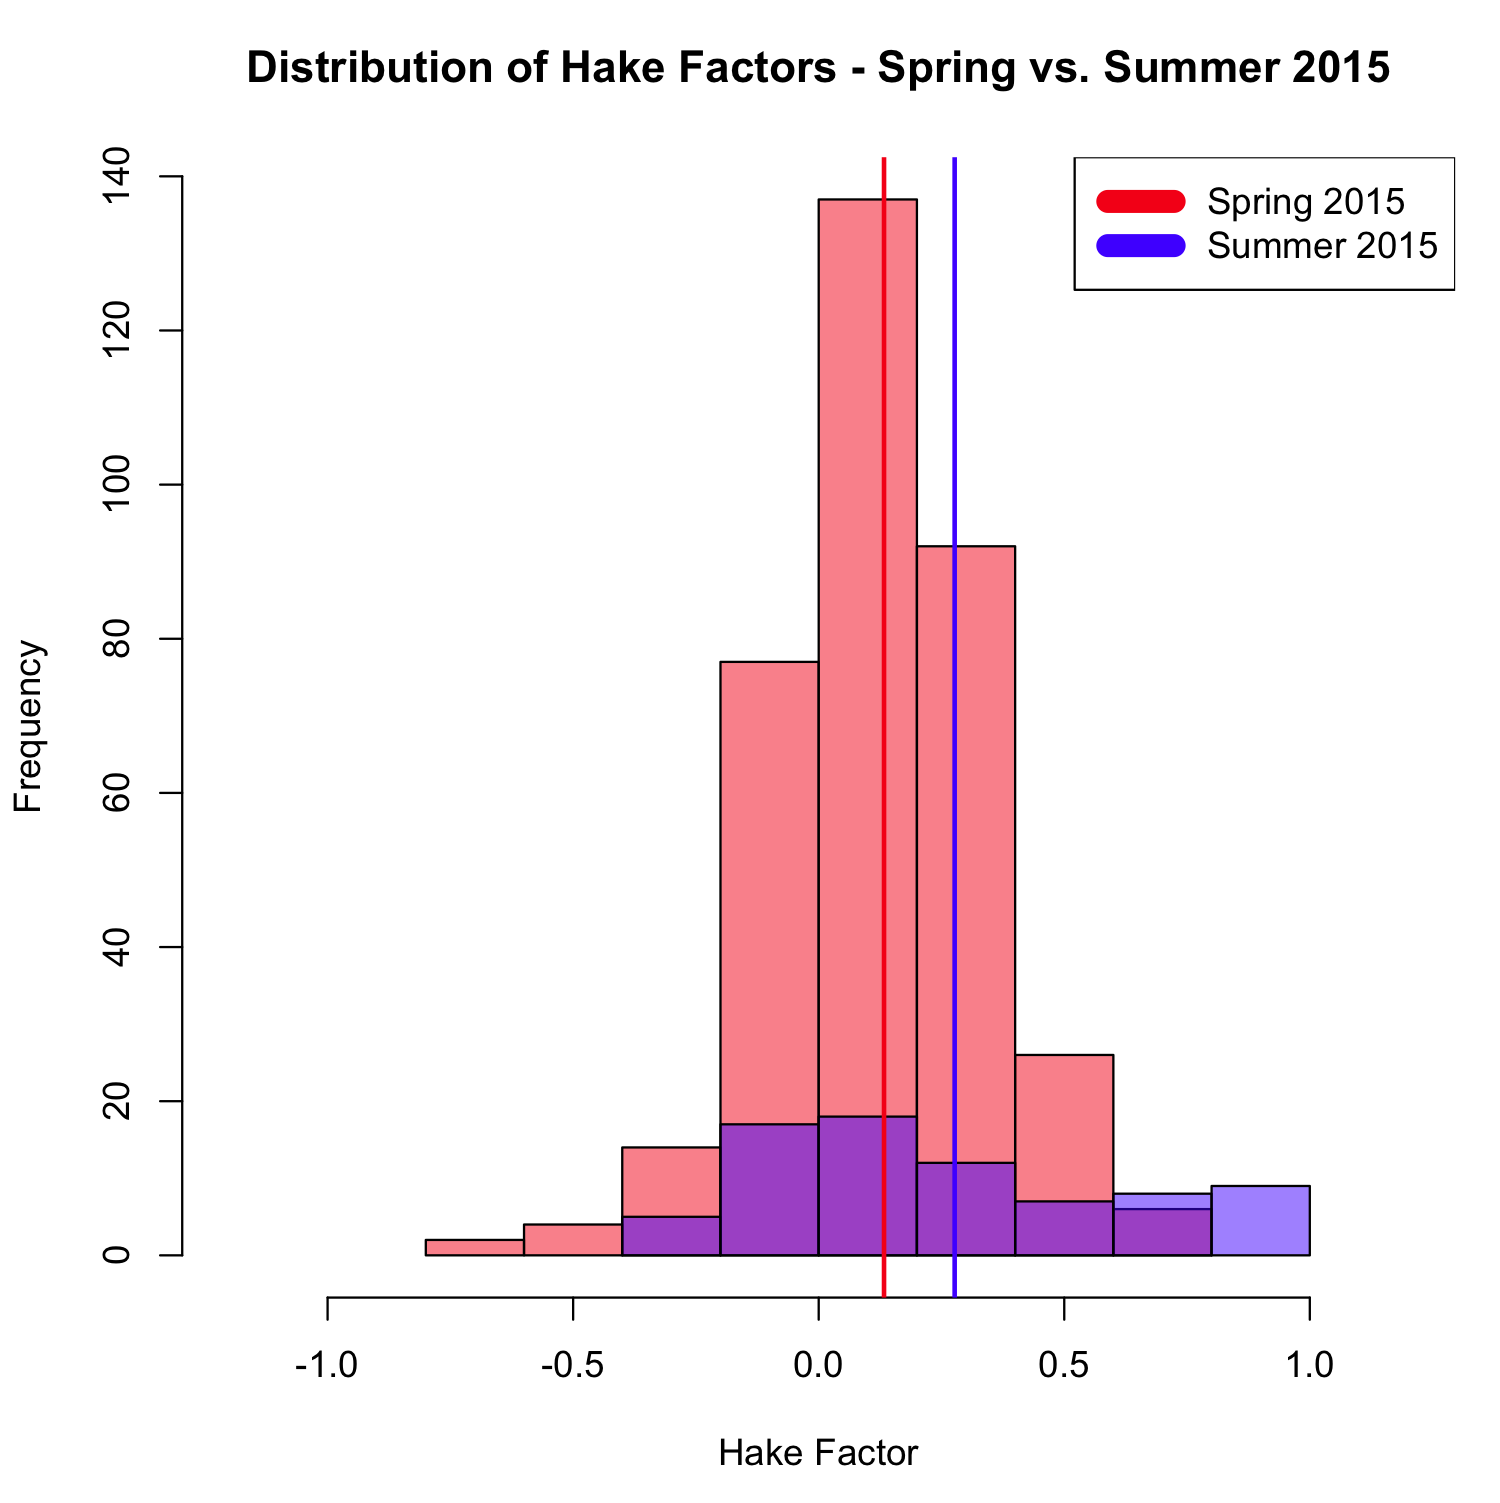
\includegraphics[width=2in]{img/chapter4/hake_spring_vs_summer_filtered}
\end{figure}
\end{column}
\begin{column}{2in}
\begin{scriptsize}
\begin{table}
  \begin{tabular}{|l|l|}
    \hline
    \textbf{Statistic} & \textbf{Value} \\
	\hline
	$\mu$ - Spring & 0.133 \\
	\hline
	$\mu$ - Summer & 0.263 \\
	\hline
	$\sigma$ - Spring & 0.208 \\
	\hline
	$\sigma$ - Summer & 0.440 \\
	\hline
	Shapiro-Wilk - Spring & p = 6.683e-05 \\
	\hline
	Shapiro-Wilk - Summer & p = 8.509e-06 \\
	\hline
	Wilcoxon Signed-Rank & p = 0.009334 \\
	\hline
	Cohen's D & 0.503 \\
	\hline
  \end{tabular}
\end{table}
\end{scriptsize}
\end{column}
\end{columns}
\end{frame}

\begin{frame}{Enrollment in Electricity and Optics}
\begin{figure}
	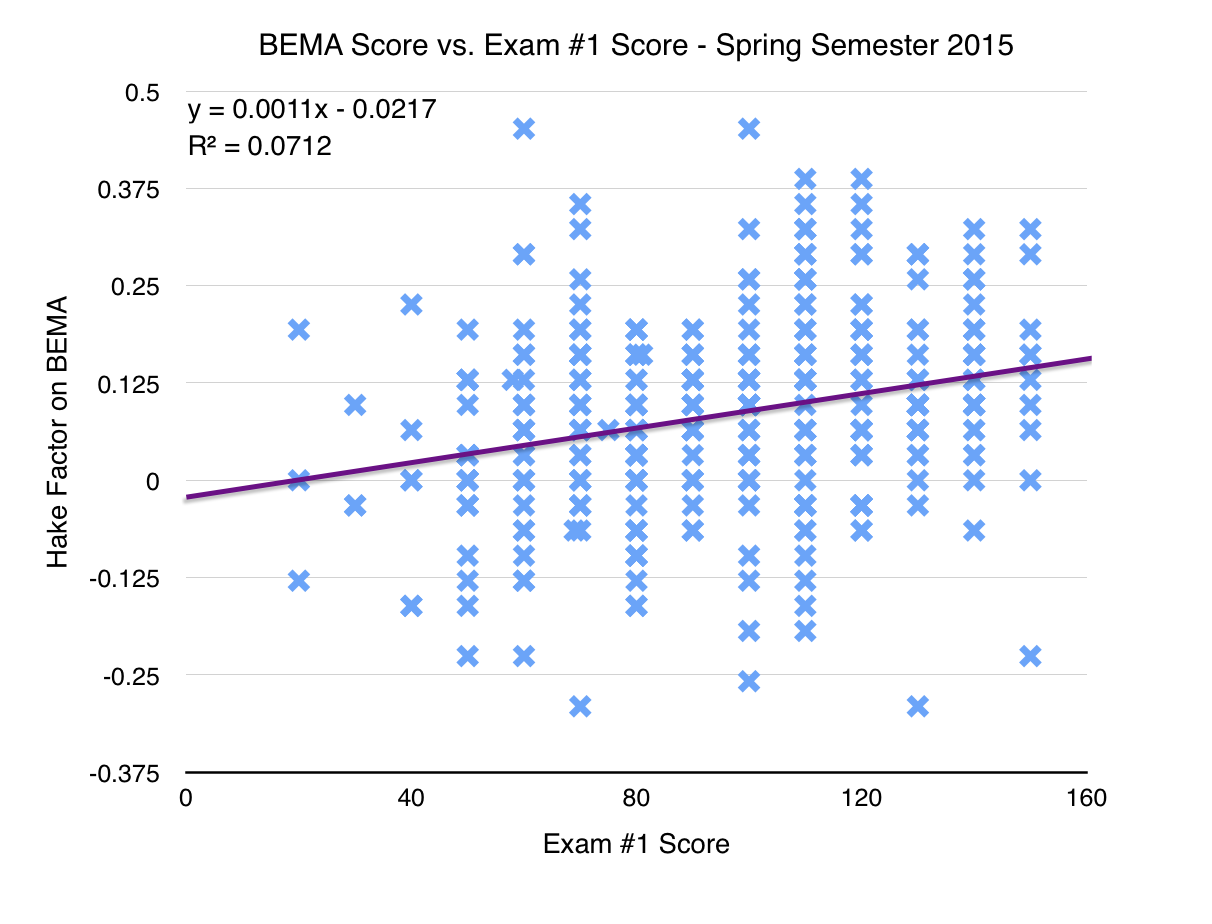
\includegraphics[width=3.6in]{img/chapter4/bema_vs_ex1_sp15}
\end{figure}
\end{frame}

\begin{frame}{Enrollment in Electricity and Optics}
\begin{figure}
	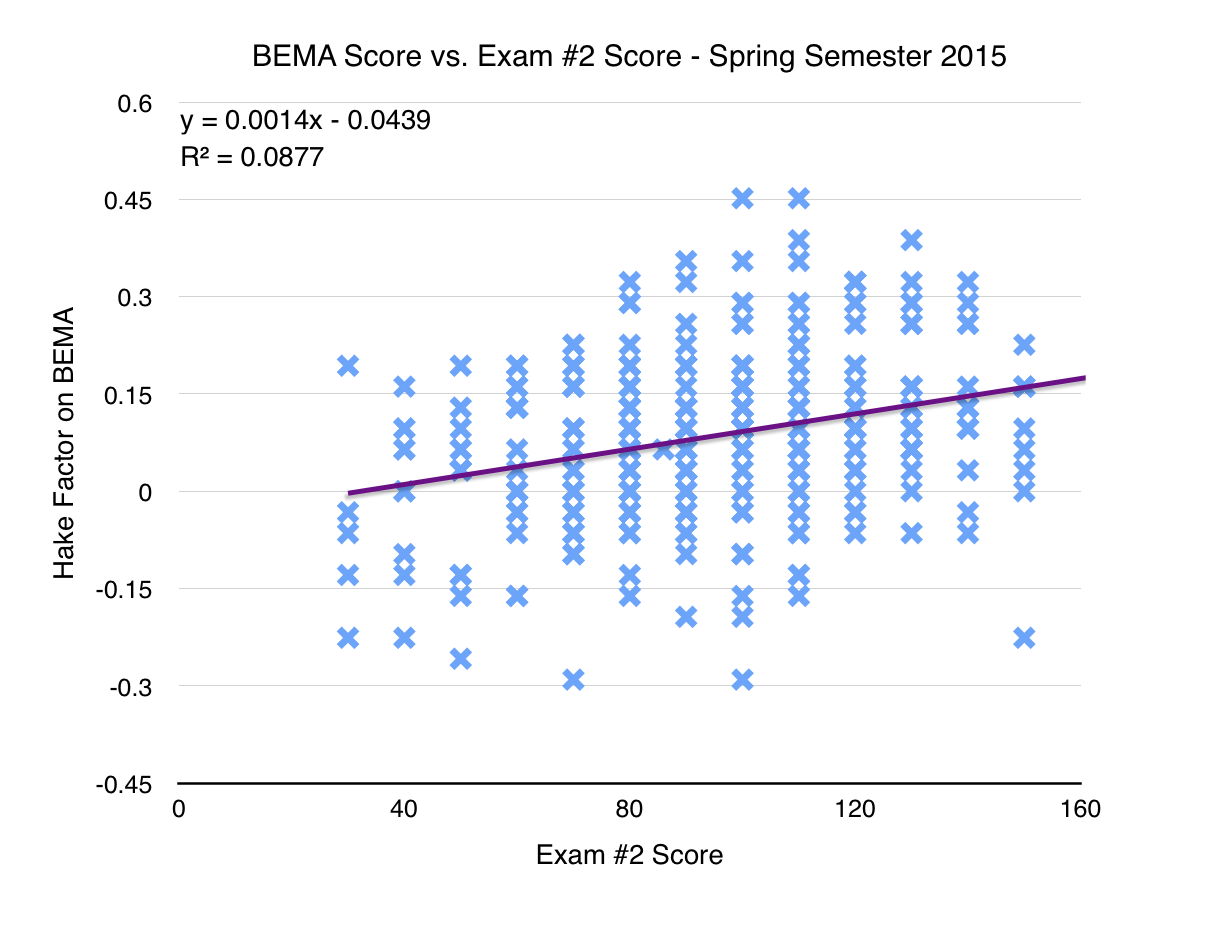
\includegraphics[width=3.6in]{img/chapter4/bema_vs_ex2_sp15}
\end{figure}
\end{frame}

\begin{frame}{Enrollment in Electricity and Optics}
\begin{figure}
	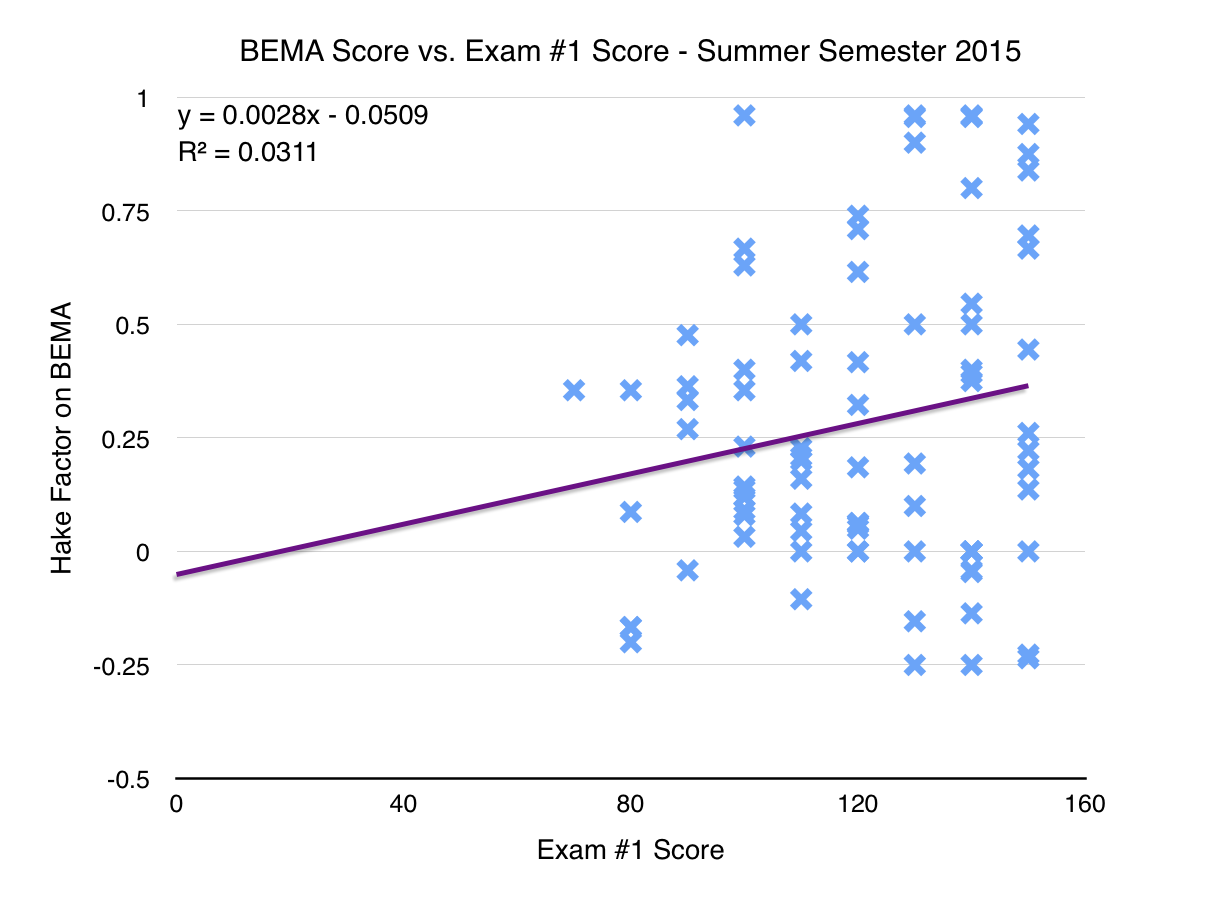
\includegraphics[width=3.6in]{img/chapter4/bema_vs_ex1_su15}
\end{figure}
\end{frame}

\begin{frame}{Enrollment in Electricity and Optics}
\begin{figure}
	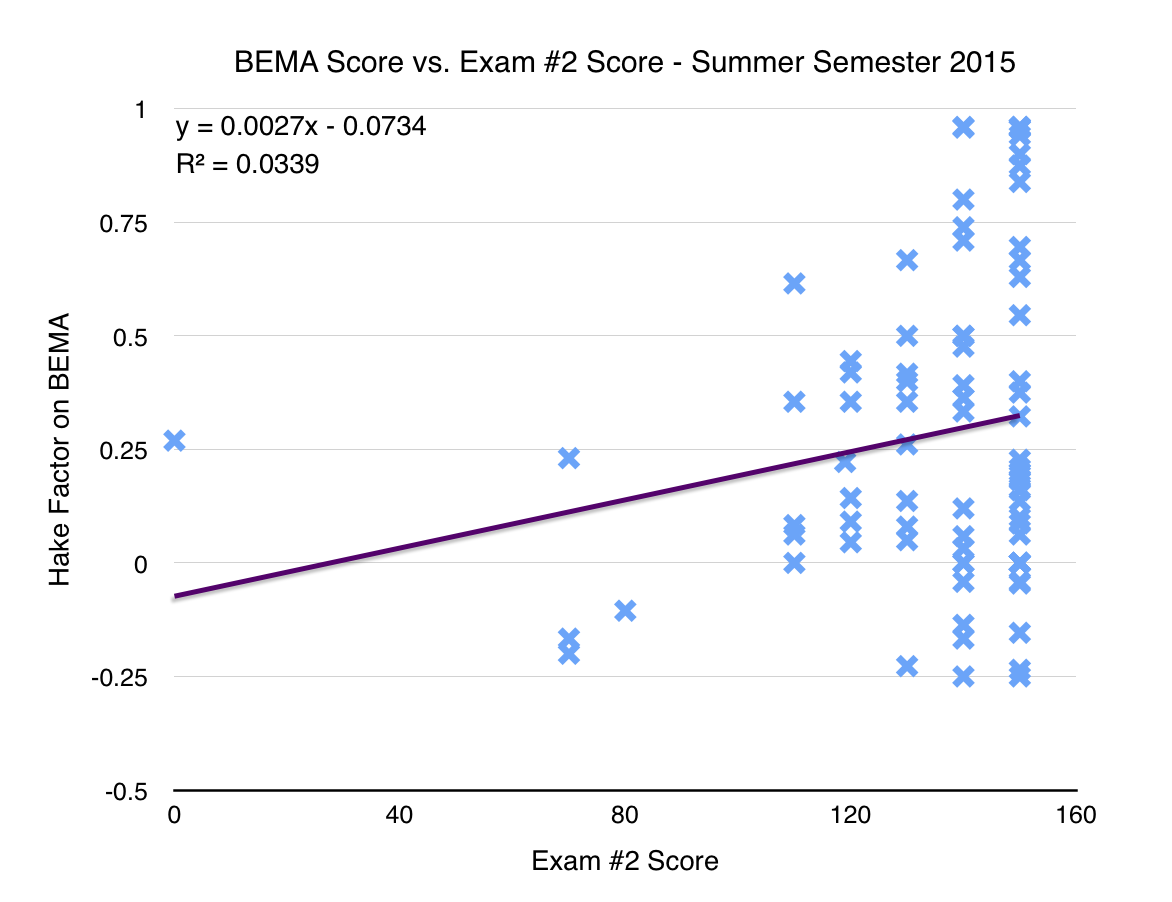
\includegraphics[width=3.6in]{img/chapter4/bema_vs_ex2_su15}
\end{figure}
\end{frame}

\section{Current Results}

\subsection{Conclusions}

\begin{frame}{Conclusions}
  \begin{itemize}
    \item Normal LaTeX class.
    \item Easy overlays.
    \item No external programs needed.      
  \end{itemize}
\end{frame}

\subsection{Future Work}

\begin{frame}{Future Work}
  \begin{itemize}
  \item We just completed a beta test of the system.
  \item We will start the initial data analysis this fall.
  \item CITA will be continuously improved.
\end{itemize}
\end{frame}

\end{document}
